\section{Variational Methods}\label{sec:3-variational}

One thing that we can do is apply variational methods to Anderson's model of the Kondo problem; as we will find, this will give us an even better picture of the physics occurring at this scale.

First, we are expecting some sort of singlet in the ground state. A trial wavefunction that represents this is:

\begin{equation}
  \ket{\psi_0} = \left[ \alpha_0 + \sum_{k<k_F,\sigma}\alpha_{\vv{k}}c^\dagger_{d,\sigma}c_{\vv{k},\sigma} \right]\ket{0}.
\end{equation}

The ket $\ket{0}$ represents a filled Fermi sea of conduction electrons, with $\alpha_0$ its amplitude. The other term in brackets represents all the possible combinations of excitations of an electron from the Fermi sea to the impurity site; this is exactly our singlet we are considering. We now consider the variational energy functional

\begin{equation}
  \tilde{E}[\ket{\psi_0}] = \frac{\braket{\psi_0 | \hat{H} | \psi_)}}{\braket{\psi_0 | \psi_0}},
\end{equation}

where we are using the Anderson model's Hamiltonian:

\begin{equation}
  \hat{H} = \epsilon_d n_d + Un_{d,\uparrow}n_{d,\downarrow} + \sum_{\vv{k},\sigma}c^\dagger_{\vv{k},\sigma}c_{\vv{k},\sigma} + \sum_{\vv{k},\sigma}\left( V_{\vv{k}}c^\dagger_{\vv{k},\sigma}d_\sigma + V_{\vv{k}}^* d^\dagger_\sigma c_{\vv{k},\sigma} \right).
\end{equation}

Here, $\epsilon_d$ is the occupation energy of the $d$-orbital of the impurity, $n_d = \sum_\sigma \epsilon_d d^\dagger_\sigma d_\sigma$ with $d^{(\dagger)}$ being the creation/annihilation operators for the impurity, $c^{(\dagger)}$ are the creation/annihilation operators for the Bloch states of the conduction electrons, and $V$ is the hybridization. Importantly, there is a potential term denoted $U$, which represents the Coulomb interaction between the two electrons in a doubly occupied $d$-orbital.

By plugging our trial wavefunction and Hamiltonian into the variational energy functional, we find:

\begin{equation}
  \tilde{E} = 2\sum_{k<k_F} \frac{\abs{V_{\vv{k}}}^2}{\tilde{E} - \epsilon_d + \epsilon_{\vv{k}}}.
\end{equation}

If we now define the \textit{binding energy} $\Delta_K \equiv \tilde{E} - \epsilon_d$, we can write

\begin{equation}
  \epsilon_d + \Delta_K = 2\sum_{k<k_F} \frac{\abs{V_{\vv{k}}}^2}{\Delta_K - \abs{\epsilon_{\vv{k}}}},
\end{equation}

where, since we are measuring all energies relative to the Fermi surface, we know that $\epsilon_{\vv{k}}<0$, meaning we can write it as $-\abs{\epsilon_{\vv{k}}}$. Now, we can convert this to the continuum in $k$, and if we assume that the hybridization $V$ is independent of $k$, we get

\begin{align}
  \epsilon_d + \Delta_K &= 2\rho \int_0^{\epsilon_F}\dd\epsilon \; \frac{-\abs{V}^2}{\epsilon - \Delta_K} \\
                        &= -2\epsilon\abs{V}^2 \ln\left( \frac{\epsilon_F}{\abs{\Delta_K}} \right).\label{eq:3-variational-1}
\end{align}

Our last assumption we can make is that the occupation energy of the $d$-orbital is much larger than the binding energy. In this case, we can neglect it from the left of Eq.~\eqref{eq:3-variational-1} and solve for it on the right to find

\begin{equation}
  \Delta_K = -\epsilon_F \exp\left[ -\frac{1}{2\rho J} \right],
\end{equation}

where we have taken $\abs{V}^2/\epsilon_d \equiv J$ as the coupling term. The important realization here is that this binding energy is negative, which indicates that our trial wavefunction, representative of the singlet state, is the one that is most likely and most preferable for the system to be in.

To go further, since this bound state is the most preferable, we would expect that $\braket{n_d} = 1$ in the case of a strong on-site potential/repulsion term $U$. In fact, calculating this, we find that

\begin{equation}
  1 - \braket{n_d} \approx \frac{\pi \Delta_K}{2\Delta} \ll 1 \neq 0,
\end{equation}

where $\Delta$ is the resonance width of the $d$-orbital. Interestingly, it is very small but not equal to one, indicating a slightly less than unity occupation. This means that there is going to be an excess of states at the Fermi surface, which corresponds to the \textbf{Kondo resonance}; see Fig.~\ref{fig:3-variational-kondoresonance}.

\begin{figure}[ht]
  \centering
  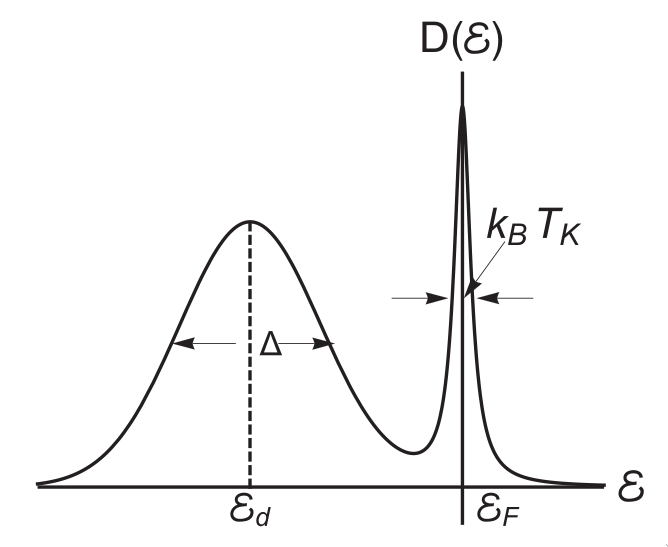
\includegraphics[width=0.5\linewidth]{./gfx/kondo-resonance.png}
  \caption{Schematic of the appearance of a Kondo resonance at the Fermi surface.}
  \label{fig:3-variational-kondoresonance}
\end{figure}

With this in mind, we can make the realization that the increased density of states is going to form a scattering center for the other conduction electrons, allowing another form of energy dissipation as the electron-phonon scattering will decrease. This explains why, after a certain temperature, the resistance starts increasing again: there is a minimum at the point when the electron-phonon interactions are very low but no singlet has formed; but, once the singlet \textit{does} form, it provides another means of scattering which will hence begin increasing the resistance again as the Kondo resonance becomes more peaked. This goes back to the Kondo cloud picture given in Fig.~\ref{fig:kondo-cloud}.




%%% Local Variables:
%%% mode: LaTeX
%%% TeX-master: "../project"
%%% End:
